\documentclass[a4paper]{exam}
\usepackage[utf8]{inputenc}

\usepackage[margin=1in]{geometry}
\usepackage{amsmath,amssymb}
\usepackage{multicol}
\usepackage{natbib}
\usepackage{graphicx}

%los de aca abajo capaz no los uso
\newcommand{\class}{Matemática: Evaluación de  Logaritmos}
\newcommand{\term}{2° Trimestre 2015}
\newcommand{\examnum}{Tema 2}
\newcommand{\examprof}{Alexis Gomel}
\newcommand{\examdate}{15/7/2015}
\newcommand{\timelimit}{60 Minutes}%no lo uso

%el header de las hojas.
\pagestyle{head}
\firstpageheader{}{}{}
\runningheader{\class}{\examnum\ - Page \thepage\ of \numpages}{\examdate}
\runningheadrule


\begin{document}
\noindent
\begin{tabular*}{\textwidth}{l @{\extracolsep{\fill}} r @{\extracolsep{6pt}} l}
\textbf{\class} & \textbf{Profesor: \examprof}\\
\textbf{\examnum} & \textbf{\examdate} \\
%\textbf{Time Limit: \timelimit} & Teaching Assistant & \makebox[2in]{\hrulefill}
\textbf{Nombre: } \makebox[2in]{\hrulefill}
\end{tabular*}\\
\rule[2ex]{\textwidth}{2pt}

%%%%%%%%%%%%%%%%%%%%%%%%%%%%%%%%%%%%%%%%%%%

Justificar cada respuesta. El examen esta pensado para que no haga falta usar una calculadora.
\begin{table}[h]
\centering
%\caption{My caption}
\label{my-label}
\begin{tabular}{|l|c|c|c|c|}
\hline
Ejercicio        & 1 & 2 & 3 & Nota \\ \hline
Puntaje maximo   & 4 & 2 & 4 &   10   \\ \hline
Puntaje obtenido &   &   &   &      \\ \hline
\end{tabular}
\end{table}

Si se traban con algún ejercicio, pasen al siguiente y vuelvan a intentar mas tarde con el que dejaron.

\\

\begin{enumerate}
\item (4 Puntos)\textbf{Resolver:} Cada ítem vale medio $0,5$ puntos.
\begin{multicols}{2}
\begin{enumerate}
\item $log(1000)-\frac{1}{2}.log_{1/3}(1)$
\item $9^{log_3(7)}$
\item $log_3(\frac{1}{27})$
\item $e^{2.ln(2) - 3.ln(4) - 3^{6}.ln(1)}$

\columnbreak

\item $\frac{1}{2}log(12+4.\sqrt{11})+\frac{1}{2}log(12-4.\sqrt{11})$

Sabiendo que $log_5(3)\simeq 0,68$, calcular:

\item $log_5(15)$
\item $log_3(5)$
\item $log_5(9)$


\end{enumerate}
\end{multicols}

\item (2 Puntos)\textbf{Gráficos:}
Cada ítem vale 1 punto.
\begin{enumerate}
\item Graficar $log_{\frac{1}{3}}(\frac{1}{3}.(x-2))$. (Basta con usar solo 4 puntos)

\item Encontrar $a$,$b$ y $c$,  a partir del gráfico de $y=log_a(c(x-b))$

\begin{figure}[h!]
\centering
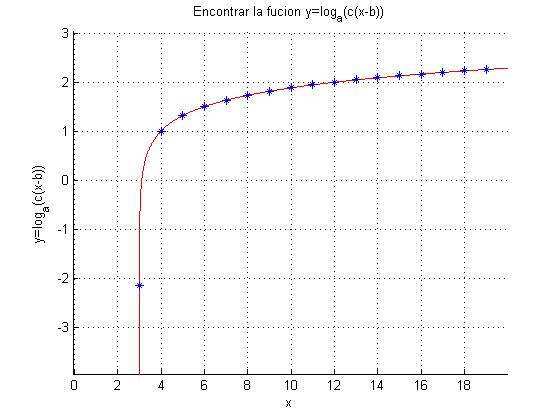
\includegraphics[width=0.6\textwidth]{logsencontrar1.jpg}
\caption{Encontrar $a$,$b$ y $c$,  a partir del gráfico de $y=log_a(c(x-b))$}
\label{fig:logaritmo}
\end{figure}

\end{enumerate}

\item (4 Puntos)\textbf{Encontrar, si es posible, el valor de x :}
Cada item vale 1 punto.
\begin{enumerate}
\item $3^x+4.3^x+3^{x+2}=126$
\item $4.log_4(x)-6.log_{16}(x)=16 $
\item $log_8(2.x-4)=1$
\item $log(x)=log(\frac{5.c}{3})-3.log(c)$
\end{enumerate}
 \\
\end{enumerate}
 \\
 \rule[2ex]{\textwidth}{2pt}
 
“There’s as many atoms in a single molecule of your DNA as there are stars in the typical galaxy. We are, each of us, a little universe.”
― Neil deGrasse Tyson, Cosmos 

%begin{figure}[h!]
%\centering
%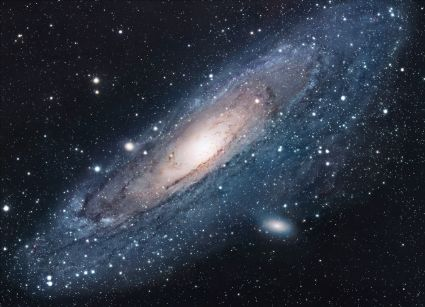
\includegraphics[scale=1.7]{universe.jpg}
%\caption{The Universe}
%\label{fig:univerise}
%\end{figure}

%\bibliographystyle{plain}
%\bibliography{references}

\newpage

\section*{Respuestas}
1: a)3 b)49 c)-3 d)$ 1/16$ e)$ 1+0,68 $ f)$ 1,46$ g)$2.0,68$ h)1

2: ver grafico

3:$log_9(9.(x-3))$

4: a)2  b)2 c)2 d)$\frac{5}{3.c^2}$

\end{document}
